%%% start preambling . . .  %%%
\documentclass{article}
% required 
\usepackage{amsmath}
\usepackage[semicolon]{natbib}
\bibliographystyle{plainnat} %{unsrtnat}
\usepackage{xr-hyper}
\usepackage{hyperref}
\externaldocument[supplement-]{supplement}
\usepackage{booktabs,siunitx}
\usepackage{Sweave}
\usepackage{graphicx}
\usepackage{lipsum}                     % Dummytext % https://tex.stackexchange.com/questions/9796/how-to-add-todo-notes
\usepackage{xargs}                      % Use more than one optional parameter in a new commands
\usepackage[pdftex,dvipsnames]{xcolor}  % Coloured text etc.
\usepackage[colorinlistoftodos,prependcaption,textsize=tiny]{todonotes}
\newcommandx{\unsure}[2][1=]{\todo[linecolor=red,backgroundcolor=red!25,bordercolor=red,#1]{#2}}
\newcommandx{\change}[2][1=]{\todo[linecolor=blue,backgroundcolor=blue!25,bordercolor=blue,#1]{#2}}
\newcommandx{\info}[2][1=]{\todo[linecolor=OliveGreen,backgroundcolor=OliveGreen!25,bordercolor=OliveGreen,#1]{#2}}
\newcommandx{\improvement}[2][1=]{\todo[linecolor=Plum,backgroundcolor=Plum!25,bordercolor=Plum,#1]{#2}}
\newcommandx{\thiswillnotshow}[2][1=]{\todo[disable,#1]{#2}}
% https://tex.stackexchange.com/questions/60209/how-to-add-an-extra-level-of-sections-with-headings-below-subsubsection
\usepackage{titlesec}
\setcounter{secnumdepth}{4}

\titleformat{\paragraph}
{\normalfont\normalsize\bfseries}{\theparagraph}{1em}{}
\titlespacing*{\paragraph}
{0pt}{3.25ex plus 1ex minus .2ex}{1.5ex plus .2ex}

% recommended! Uncomment the below line and change the path for your computer!
 
%put your figures in one place! Also, note that here 'figures' is the folder and 'demoFig' is what each 
% figure produced will be titled plus its number or label (e.g., demoFig-nqpbetter.pdf')
% make your captioning look better
\usepackage[small]{caption}
\setlength{\captionmargin}{30pt}
\setlength{\abovecaptionskip}{0pt}
\setlength{\belowcaptionskip}{10pt}
% optional: muck with spacing
\topmargin -1.5cm        
\oddsidemargin 0.5cm   
\evensidemargin 0.5cm  % same as oddsidemargin but for left-hand pages
\textwidth 15.59cm
\textheight 21.94cm 
% \renewcommand{\baselinestretch}{1.5} % 1.5 lines between lines
\parindent 0pt		  % sets leading space for paragraphs
% optional: cute, fancy headers
\usepackage{fancyhdr}
\pagestyle{fancy}
\fancyhead[LO]{March 2023}
\fancyhead[RO]{Manuscript}
% more optionals! %
% \usepackage[hyphens]{url} % this wraps my URL versus letting it spill across the page, a bad habit LaTeX has
%%% end preambling. %%%

\begin{document}
\Sconcordance{concordance:supplement.tex:supplement.Rnw:%
1 65 1}
 % For RStudio hiccups
\title{{\huge Changes and trends in budburst and leaf flush across Europe and North America} \\A meta-analysis of local adaptation in spring phenology studies}
\author{Ziyun Zeng \& E. M. Wolkovich}
\date{2023}
\maketitle 


\newpage

\section*{Abstract}


We conducted the first cross-continental meta-analysis of published studies from the peer-reviewed literature that reported spring event dates for a mix of angiosperm and gymnosperm tree species in the northern hemisphere, capturing data from 384 North American provenances and 101 European provenances with observations from 1962 to 2019.


\section{Introduction}
\begin{itemize}
\item Define spring event, fall event
\item Background
\item Importance: An accurate understanding of how species distribution might be influenced by environmental conditions at a continental scale is critical for future range shift prediction. 
\item Knowledge Gap: Anecdotally, the spring phenology of trees from European provenances appeared to exhibit stronger clines and less plasticity than in North American studies. Despite a growing interest in predicting local adaptation across locations, no study has comprehensively examined clines for spring and fall events and what factors may underlie differences observed across studies.
\item Research question (links to results)
\end{itemize}

We ask: Across common garden studies, how strong are clines in spring and fall phenology?

To better understand these clines, we also aim to examine:
\begin{itemize}
\item If differences in clines exist across Europe and North America.
\item If differences in clines exist across angiosperm and gymnosperm species.
\item If climate overlap (see Figure 1) between the provenance and garden explains the similarities and differences in clines.
\end{itemize}
To our knowledge, this marks the first study to synthesize spring phenology data retrieved from studies across North America and Europe. 


\subsection*{Ref notes}
\todo[inline]{Good background information.}

\citep{AitkenBemmels16}\\
"Geographic variation in trees has been investigated since the mid-18th century. Similar patterns of clinal variation have been observed along latitudinal and elevational gradients in common garden experiments for many temperate and boreal species."\\
"Scientists have studied relationships between tree populations and environmental characteristics of their provenances in common garden experiments for over 250 years."\\
\\
\citep{Alberto13}\\
"Evolutionary responses are required for tree populations to be able to track climate change. Results of 250 years of common garden experiments show that most forest trees have evolved local adaptation, as evidenced by the adaptive differentiation of populations in quantitative traits, reflecting environmental conditions of population origins."\\
"Thus, responding to climate change will likely require that the quantitative traits of populations again match their environments. We examine what kind of information is needed for evaluating the potential to respond, and what information is already available. We review the genetic models related to selection responses, and what is known currently about the genetic basis of the traits. We address special problems to be found at the range margins, and highlight the need for more modeling to understand specific issues at southern and northern margins. We need new common garden experiments for less known species. "\\
"Modeling work on the potential of populations and species to respond genetically to recent climate change is advancing (see Hoffmann \& Sgrò, 2011; Franks \& Hoffmann, 2012; Shaw \& Etterson, 2012 for recent reviews). "\\

(see e.g., Valladares et al., 2007; Caffarra et al., 2011; Hänninen \& Tanino, 2011)
"The plastic response of different traits (e.g., phenology in trees) to variation in climate is, however, often much more complex than in heuristic models of adaptation."\\


\citep{Loarie09}\\ 
"It is also now understood that the rate of adaptation required by climate change varies among geographic regions." \improvement{need to read again}\\

\citep{Nicotra10}\\ 
"The immediate responses via phenotypic plasticity have also been considered in the context of climate change." \improvement{need to read again}\\

\citep{Menzel99} \textbf{Growing season extended in Europe.}\improvement{good Europe background paper}\\
\citep{Menzel06} \textbf{European phenological response to climate change matches the warming pattern.}\improvement{another good Europe background paper}\\
\citep{Parmesan06}\\
"Trees exhibit a high degree of phenotypic plasticity with respect to climatic variation. Phenological shifts of bud flush in response to recent increases in temperatures have been widely documented ." \improvement{can cite more papers on this matter}


\citep{Gill15} \textbf{Changes in autumn senescence in northern hemisphere deciduous trees: a meta-analysis of autumn phenology studies.} \improvement{GREAT paper for us to base our writing on: similar meta-analysis but focuses on fall events}\\
"the effects of climate change on the phenology of vegetation have received increased attention over the past several decades as any factor that alters the timing of early growing season leaf-out and senescence has the potential to affect a variety of ecosystem properties. For example, the timing of leaf-out and senescence of deciduous plants has been shown to affect plant competition (Fridley, 2012), plant growth (Myneni et al., 1997) and ecosystem carbon uptake (Barichivich et al., 2012).\\

"While leaf-out has been shown to advance over the past century as a result of increasing air temperatures (Linderholm, 2006; Polgar and Primack, 2011), the relationship between temperature and leaf senescence remains less well understood (García-Plazaola et al., 2003; Richardson et al., 2013)."

"Thus, an extension of the growing season can contribute to reduced atmospheric CO2 concentrations due to enhanced carbon sequestration in terrestrial plants (Penuelas et al., 2009; Richardson et al., 2013). However, the increase in carbon uptake may be partially offset by increased rates of ecosystem respiration (Piao et al., 2008)"

"The lack of consistent relationships between air temperature and timing of leaf senescence suggests that autumn senescence may be influenced by a variety of factors that obscure its relationship with temperature."


\todo[inline]{Cite some papers about the documented trends}

tbc...

 
 

\todo[inline]{Alina says: I found AitkenBemmels2016's research question to be wonderfully phrased and think we can do something similar}
\citep{AitkenBemmels16}\\
"To what extent are patterns of local adaptation along climatic gradients similar among species within a given geographic region? If clines in phenotypic traits are similar, can average patterns of sympatric variation guide AGF or identify critical climatic variables as a first approximation for untested species? We reanalysed data from the literature on provenance trials in temperate tree species from western North America to address these questions. This is an ideal region of focus because of the many provenance trials conducted on native tree species that are important for forestry, and because its high topographic complexity means that turnover in climate occurs rapidly and heterogeneously over short geographic spaces. Clines along climate gradients are thus espcially likely to reflect local adaptation to climate, rather than non-adaptive phenomena resulting from population demographic history."
\\

% alina_Jan27 -- I think we should have a section to define "spring events, fall events, distance between garden locations, difference of latitude, etc. Where do you think this section should go? Methods? EMW replies -- I think defining the events would be good, distance between garden locations and latitude etc should be SHORT (for example we use XX R package to calculate yy). I would put all this in the methods. The definition of events can go in the dataset assembly and I would start a section on 'analyses' where you include most of 2.3 *and* 2.4. I would move up where you got climate data from to above -- think of a 'Data' section with some subheaders and an 'analyses' section with some subheaders. 

% I am pasting a paragraph of the method section of Ettinger below to make reference to later on when I write the definition section. 
"Defining budburst. Most studies defined budburst as initial ‘green tips’ (33 out of
49 papers). Select studies defined budburst as a specific increment of growth (for
example, ‘0.5 cm of new growth’) or as bud swell, leaf emergence, leaf unfolded,
open bud scales or petiole emerged. The remaining papers (4 of 49) did not
include a definition of budburst. Most papers using the above definitions (34 of 49)
required only one bud to have met the defined criteria of budburst; however, the
remaining studies implemented specific thresholds to be met (10–100\% of all buds
on an individual needed to have bursted bud). For studies that quantified multiple
measurements of percentage budburst over time (days), we extracted one value of
‘days to budburst’ of these multiple measurements to make them comparable to
other studies. To extract this summary value, we selected the days to budburst when
percentage budburst was closest to 90\%, including estimates as low as 49.5\% budburst"

%emw6Mar -- below opening and questions are good, but not appropriate for results. Move up to be at end of introduction. 
\verb@Research questions recap@
\\
Despite a growing interest in predicting local adaptation across locations, no study has comprehensively examined clines for spring and fall events and what factors may underlie differences observed across studies.

We ask: Across common garden studies, how strong are clines in spring and fall phenology?

To better understand these clines, we also aim to examine:
\begin{itemize}
\item If differences in clines exist across Europe and North America.
\item If differences in clines exist across angiosperm and gymnosperm species.
\item If climate overlap between the provenance and garden explains the similarities and differences in clines.
\end{itemize}

\section{Methods}
\subsection{Data Collection}
%emw2Mar: Try to open with WHY (goal/aim) you did something more than what you did, not a rule, but try to do when possible. 
To locate common garden studies that documented the timing of spring events of woody plant species we searched and reviewed the peer-reviewed literature. On 14 December 2022 we searched Web of Science (Thompson Reuters, New York, NY) using the following terms:
\begin{quote}
TOPIC = (common garden* OR provenance*) AND (leafout* OR leaf out* OR budburst OR spring phenolog*)
\end{quote}
which returned 122 publications. We also contacted authors of previous review papers \citep{AitkenBemmels16, Alberto13}, to help further search the literature. We then reviewed the methods and results of all publications to refine to only studies that met the following criteria: (a) focused on woody plants originating from either Europe or North America, (b) had provenance trials/common gardens on the same continent, (c) reported spring events in units of calendar days (day of year or DOY) or could be converted into DOY (see `Additional Methods' section in the Supplement), and (d) reported latitude and longitude of provenances and gardens. 
\\
\\
Based on these criteria we found 18 provenance/common garden studies, distributed throughout North America and Europe, with the majority of data concentrated in North America (Figure X). From each paper we extracted phenological data on spring events (budburst and leaf flush in DOY) and, when present in the same paper, fall events (bud set, leaf senescence, growth cessation, and leaf abscission) by species, provenance and garden location (geographic coordinates). We used ImageJ (version 1.53k; \citealp{schneider_rasband_eliceiri_2012}) to extract values from figures whenever necessary. For studies that reported event dates relative to a reference date other than 1 January (e.g. \citealp{Rehfeldt1994}), we converted such dates to DOY using the Lubridate Package in R.
\improvement{display a table and a map here, and in the caption, clarify that some studies had more than one gardens and two studies shared the same garden}
%emw2Mar -- mv the following sentence to the caption of the map figure: The distribution was skewed toward North America (n = X), with only X located in Europe. %alinaMar5:think abt displaying number of studies or provenances
\\
\\
To understand how climatic differences, in addition to geographical differences, shape local adaptation in spring events we extracted several types of climate data using information about provenance latitude, longitude, and elevation from original publications. We estimated the mean annual temperature (MAT) for each provenance using the Climate Information Tool by Food and Agriculture Organization of the United Nations \citep{FAO2022}and ClimateWNA \citep{wang2016}. To examine more explicitly climate near spring events, we used gridded daily temperature data for 2011 to 2020 for all European and North American provenances and gardens from E-OBS and the daymetr R package respectively \citep{cornes2018,hufkens2018}. Using these data we estimated how much the daily temperatures overlapped between garden and provenance locations, which we call `climate overlap.' For this we used the Overlap package in R to calculate the percentage overlap of the daily temperature of each provenance in spring months (March to May) from 2011 to 2020 in relation to the daily temperature of their corresponding gardens. Finally, using the daily data, we also calculated Growing degree days (GDD), a commonly used heat accumulation measure to forecast phenological development in plants (Miller et al., 2001), based on the accumulation of mean daily temperatures ($T_{m}$)from 2011 to 2022 above a baseline of 0$^{\circ}$C, from January 1 until budburst and leaf flush with the following formula: GDD = $\sum$($T_{m}$ - $0^{\circ}$C for $T_{m}$ $\ge$ $0^{\circ}$C; 0 for $T_{m}$ $\le$ $0^{\circ}$C).

\subsection{Analyses}
To estimate clines in spring and fall phenological events across species we used hierarchical Bayesian models. We regressed day of year (DOY) of events against geographical and climate predictors with partial pooling (sometimes called `random effects') on the intercept and slope for each species within each garden. Because most tree species were present in only one common garden in our dataset, it was impossible to fit garden and species separately, thus we treat each species within a garden as a unique group. Using posterior estimates for each species within a garden, we estimated effects of continent (North America vs. Europe) and species type (angiosperm vs. gymnosperm). All models were fit in rstanarm package (version 2.21.3; \citealp{brilleman2018}), using default priors, with 4 chains and 1000 sampling iterations per chain for a total of 4000 samples. We checked for model fit by ... [ADD here]. We present estimates as mean $\pm$ 90\% uncertainty intervals given parenthetically, unless otherwise stated. 
%emw2Mar -- It would be good if you have tidy code you can post with the data so folks can fit the models themselves. 
%emw2Mar -- Did you use default priors? If so, can you figure out how to increase them threefold and see if answers change (they change run to run, but should not change dramatically)? Ideally they don't and then we can add 'increasing priors three-fold did not change results.'

\section{Results}
%emw24Jan -- below is great opening!
%emw6Mar -- results are in past tense generally
Our final dataset captured seven angiosperm and eight gymnosperm species from 19 common gardens, encompassing 384 North American provenances and 101 European provenances, with observations from 1962 to 2019. Seven species also had fall event information available. 
\\

\todo[inline]{add map here}
\todo[inline]{add a table documenting studies attributes} %emw6Mar -- Tables should go in supplement. But we should add estimates to statements we make throughout. These should be added as mean +/- 90% uncertainty (posterior) intervals (UI) parenthetically using /Sexpr so they update automatically. 


Overall, spring events were not related to provenance latitude (0.10 days/degree [-0.06 - 0.26]) or MAT (-0.09 days/degree [-0.36 - 0.18]) in North America. \todo{add figure here} Spring events advanced slightly with provenance latitude (0.10 days/degree [-0.23 - 0.42]) and MAT (-0.16 days/degree [-0.55 - 0.23]) in Europe, meaning spring events are slightly earlier where provenance MAT is lower (i.e., higher, more northern latitudes)(Fig. \ref{figure:springfall_latmat} \& Supplement Table. \ref{supplement-table:model_sf_lat}), though uncertainty intervals strongly overlapped zero. Results were similar using other distance metrics in lieu of latitude (see Supplement Fig.\ref{supplement-figure:lat_distance} for results using the absolute value of the distance and the spherical distance difference between provenance and garden latitude). 

\begin{figure}[!h] 
    \centering
 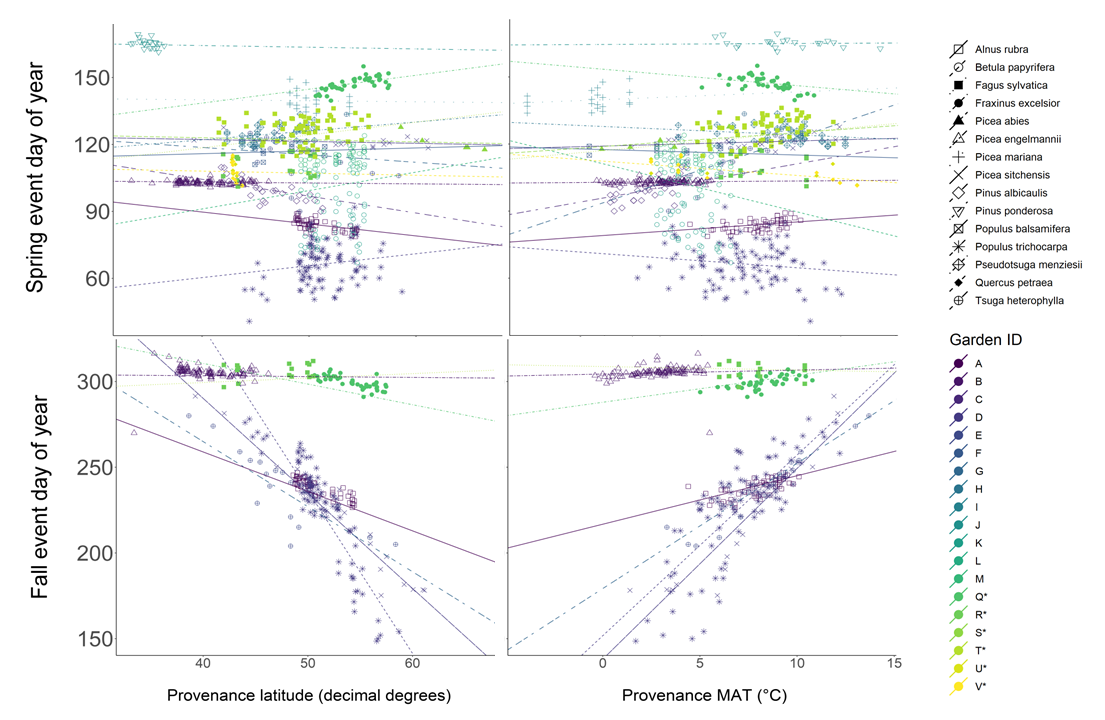
\includegraphics[width=\textwidth]{..//..//localadaptclim/Docs/figure_ms/springfall_latmat.png}
    \caption{Spring event Day of Year (DOY) in relation to provenance latitude and MAT, coded by symbol for species and color for garden with linear fits from hierarchical Bayesian models. Spring events shown on top and fall event at the bottom.} 
    \label{figure:springfall_latmat}
\end{figure}


In contrast, fall events (budset, leaf senescence, leaf abcission) advanced strongly with provenance latitude and MAT, meaning fall events are earlier where provenance MAT is lower. This relationship, however, was observed mostly in North America where fall events advance 4.24 (3.95 - 4.53) days per degree northward, or 6.41 days (5.78 - 7.04) per degree decline in MAT$^{\circ}$C (Fig. \ref{figure:continent}). In Europe, such relationship is weak: advance 0.47 (0.21 - 1.17) days per degree northward, or 0.70 days (1.04 - 2.42) per degree decline in MAT $^{\circ}$C(Fig. \ref{figure:continent}). 

\begin{figure}[!h] 
    \centering
 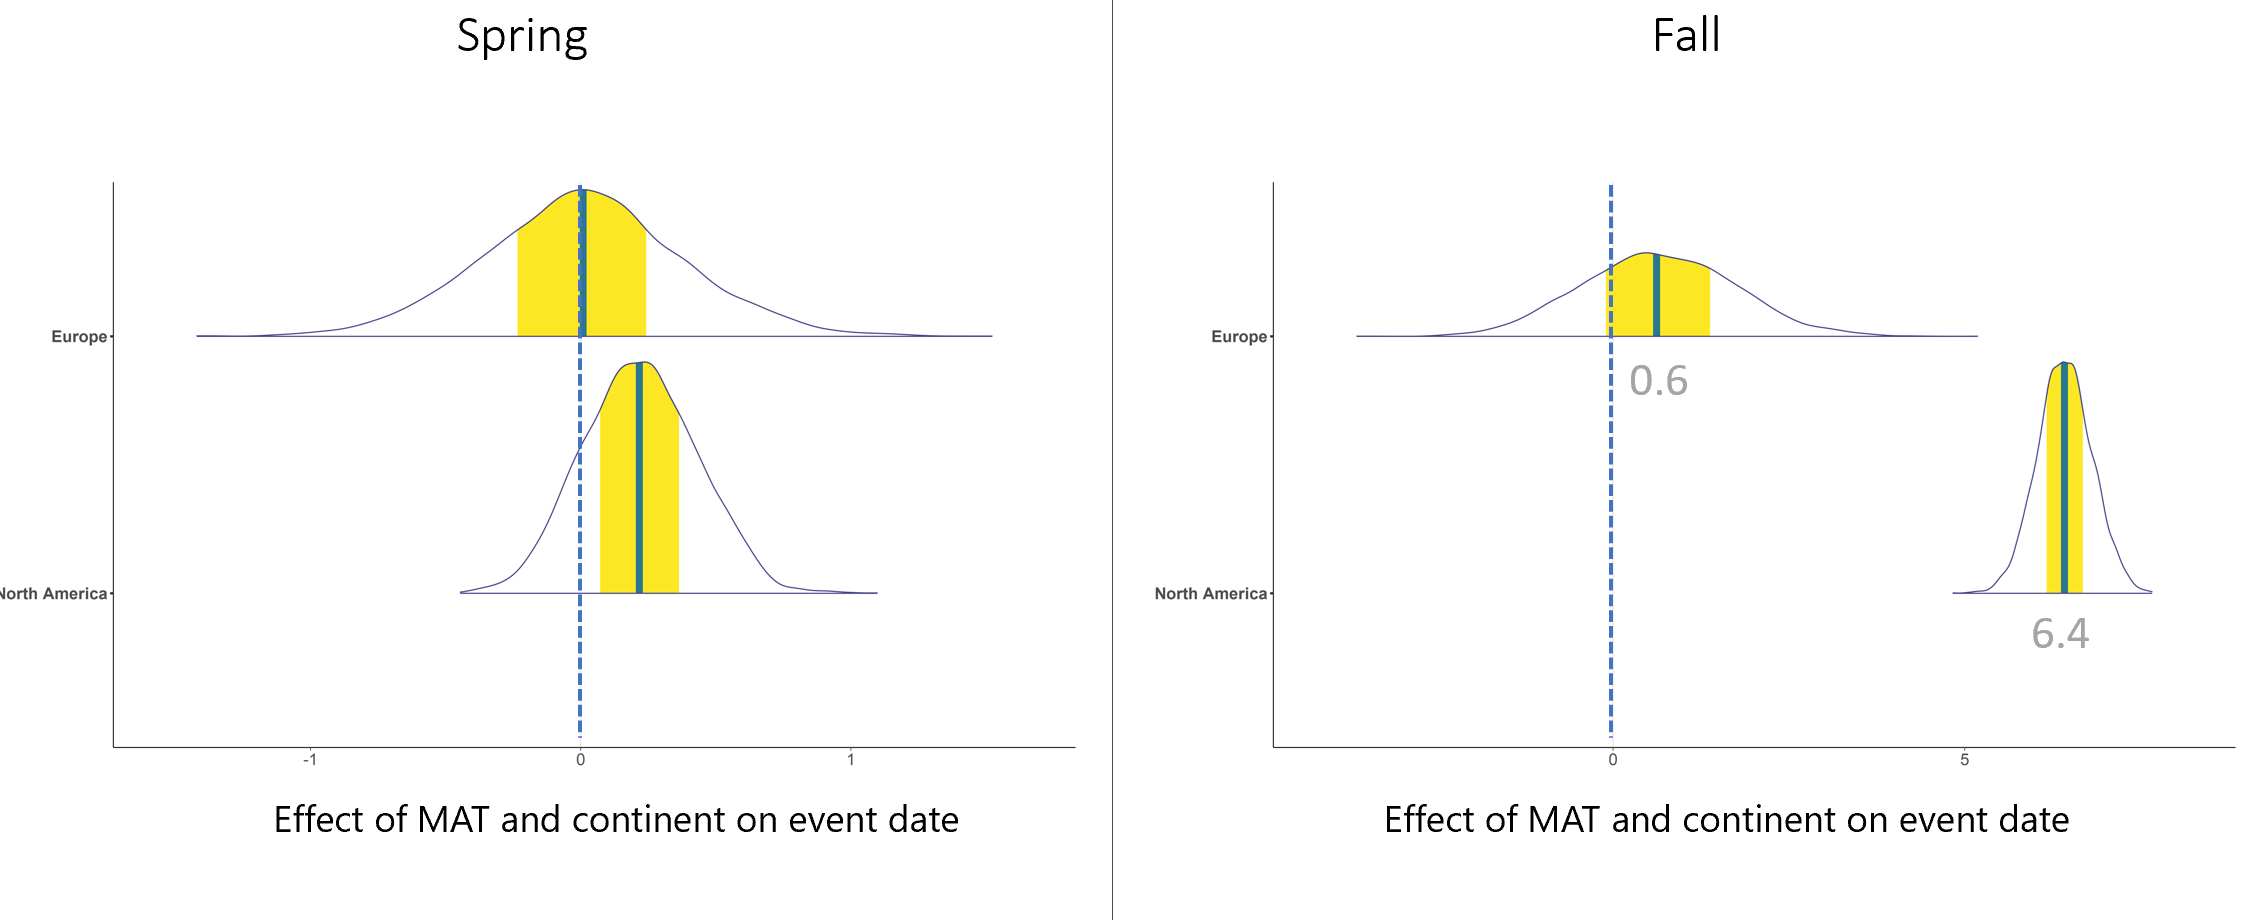
\includegraphics[width=\textwidth]{..//..//localadaptclim/Docs/figure_ms/continent_histogram.png}
    \caption{Caption placeholder}
    \label{figure:continent}
\end{figure}

Effects of provenance latitude on both spring and fall events were similar across angiosperms and gymnosperms. However, effects of MAT on spring events weakly diverge: spring events get earlier as MAT increases in angiosperms and delay as MAT increases in gymnosperms, except for \emph{Pseudotsuga menziesii}. Fall events delay in warmer locations for both species types, but slightly more so for gymnosperms (3.69 days VS. 6.23 days)(Fig. \ref{figure:spp_type}).

%(3.7 days VS. 6.2 days) 

We also tested whether climate effects on events may be stronger using metrics from seasonal windows closer to event dates, but results were not qualitatively different than using MAT. We observed very weak effects of climate overlap on spring events, nearly identical across angiosperms and gymnosperms. Fall events diverge as climate overlap declines for both angiosperms and gymnosperms, but slightly more strongly for gymnosperms (Fig.\ref{figure:overlap}).

%emw6Mar -- I think we can skip subheaders in the results (yay!) but I need to read it again once you had added all the numbers and intervals. 
\begin{figure}[!h] 
    \centering
 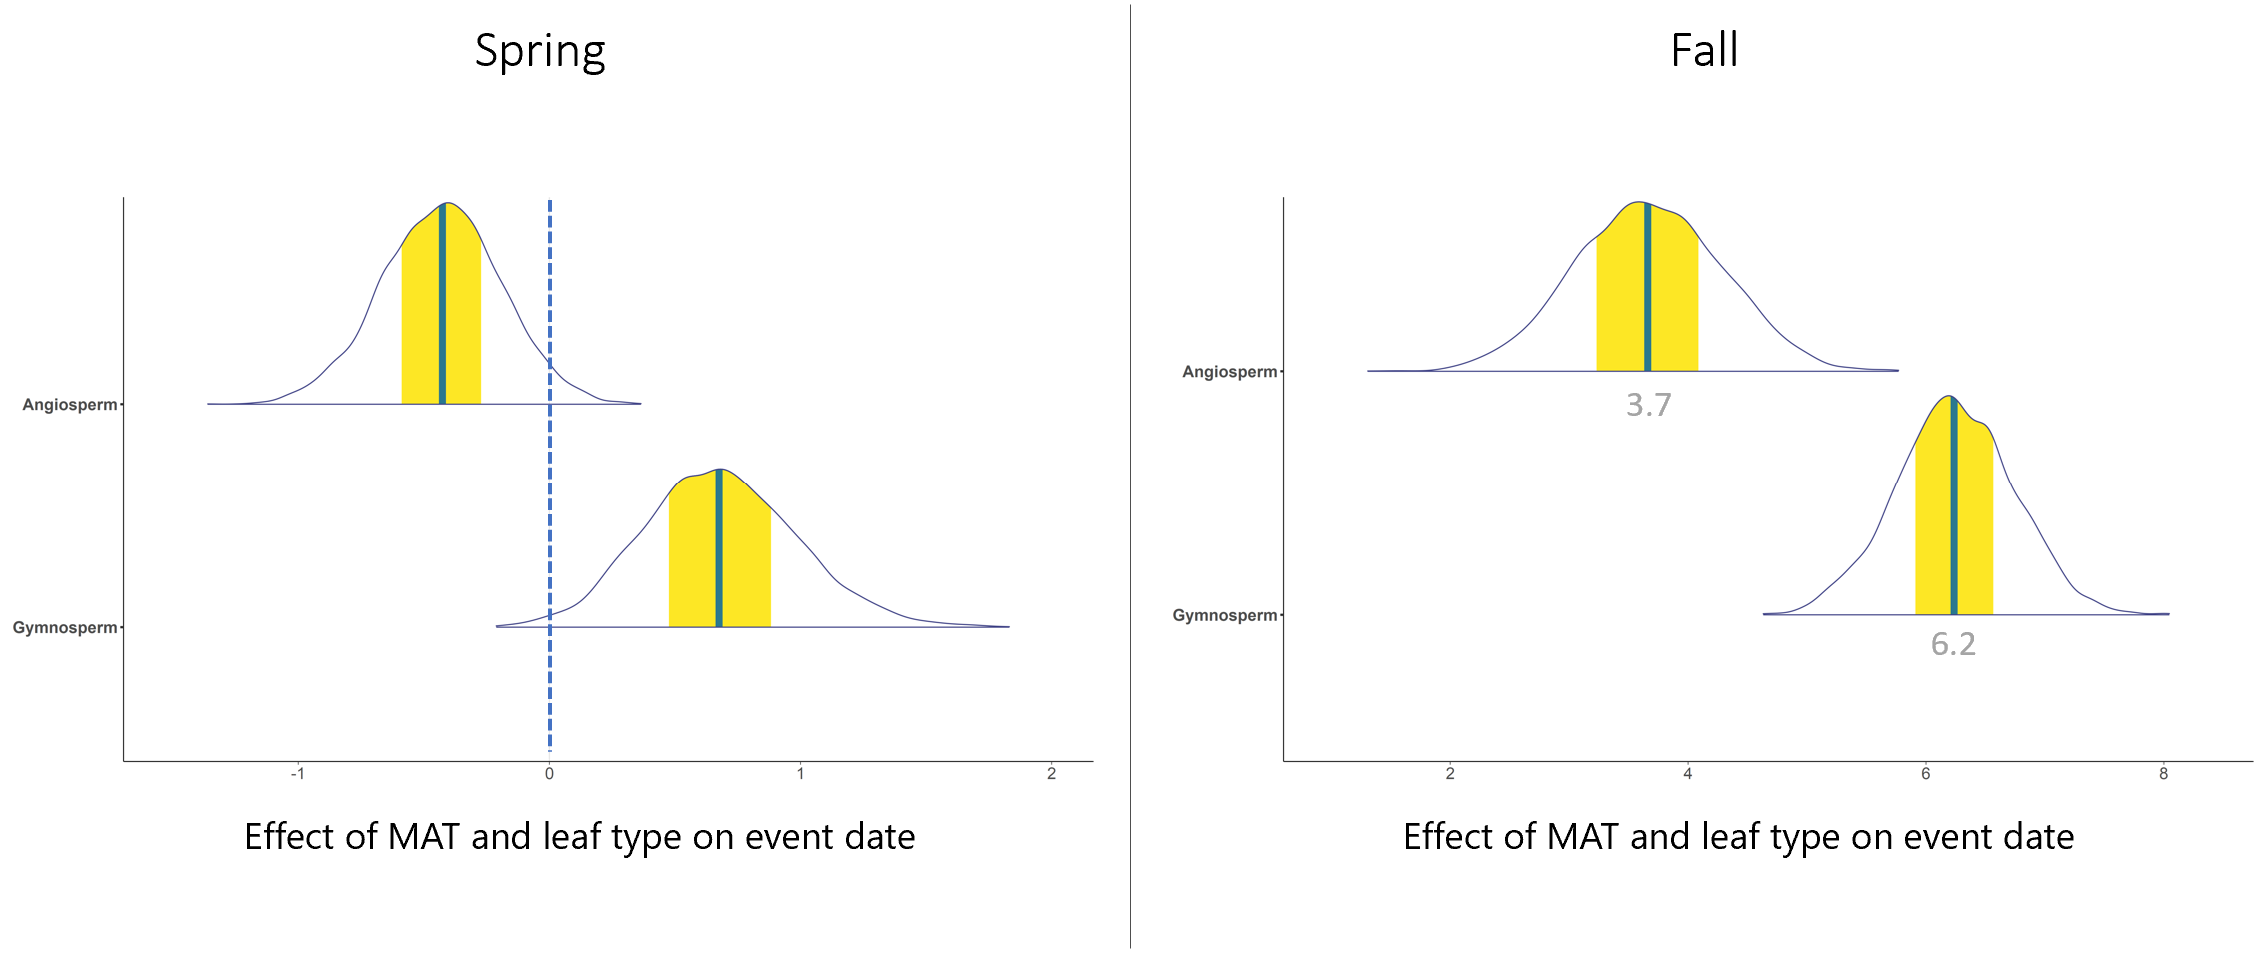
\includegraphics[width=\textwidth]{..//..//localadaptclim/Docs/figure_ms/spp_type_histogram.png}
    \caption{Caption placeholder}
    \label{figure:spp_type}
\end{figure}


\begin{figure}[!h] 
    \centering
 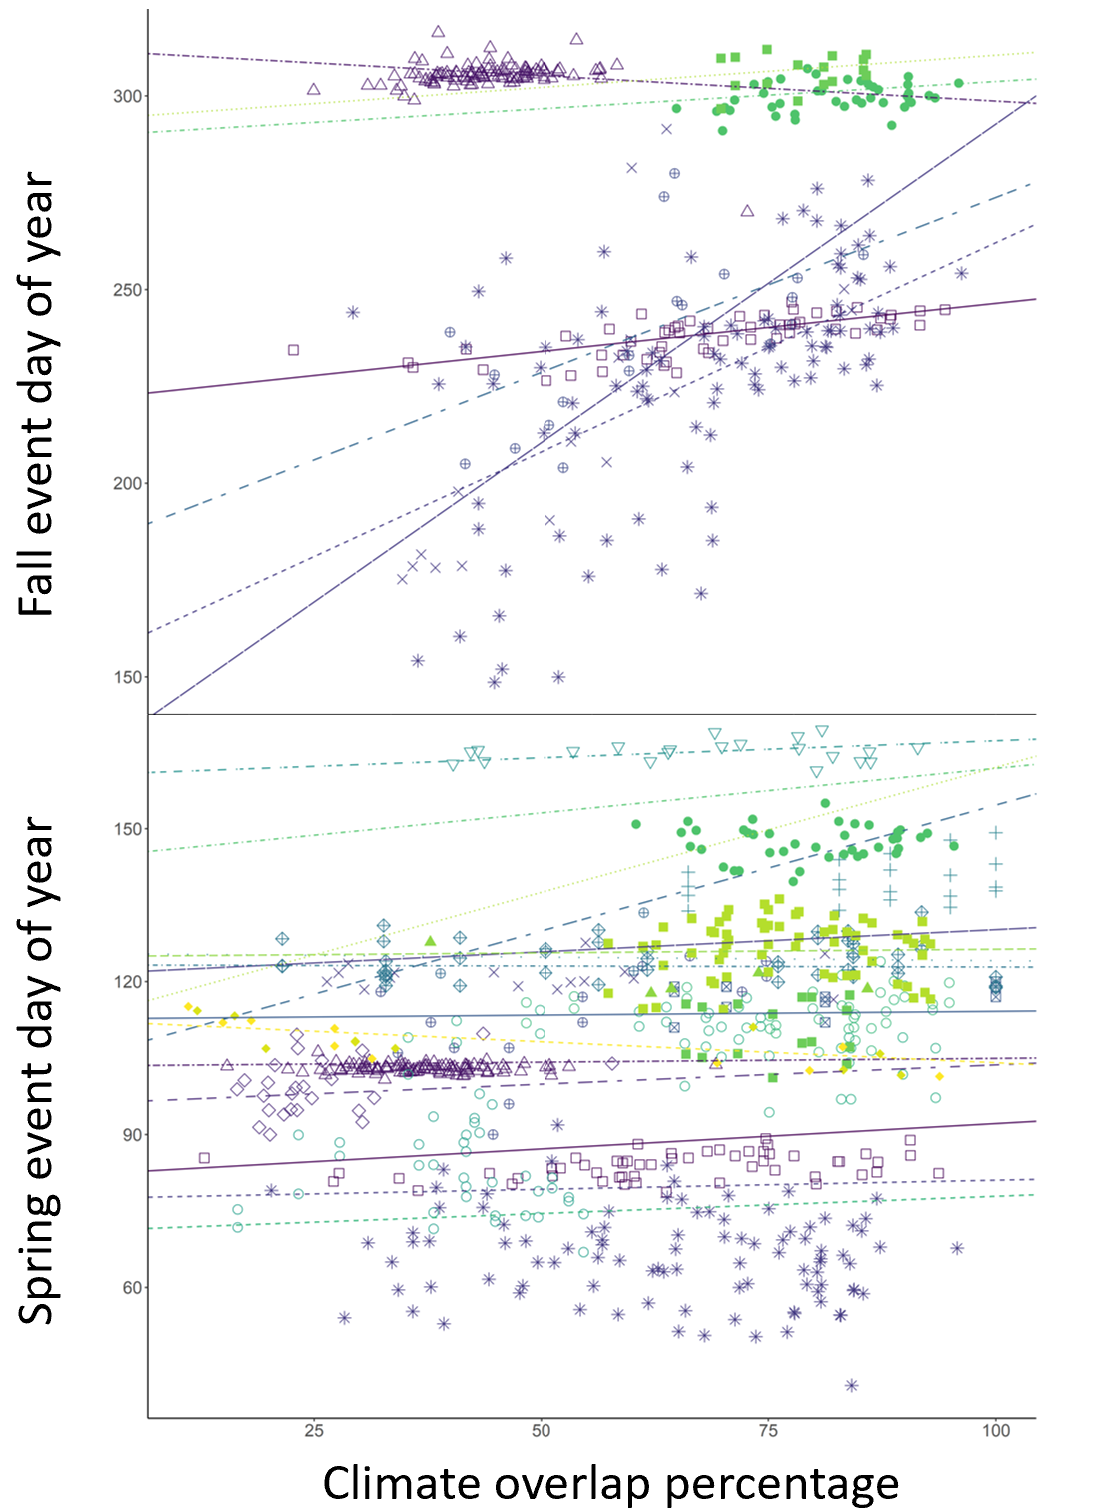
\includegraphics[width=\textwidth]{..//..//localadaptclim/Docs/figure_ms/climate_overlap.png}
    \caption{Caption placeholder}
    \label{figure:overlap}
\end{figure}
%emw6Mar -- Climate overlap figures can go in supp. 

%emw6Mar -- I could combine the current fig 3-4. Just be sure to label each panel. 


% old graphs can be found in C:\Users\alina\Documents\git\localadaptclim\Output\plotMay15_two predictors_experiment
% refer to analyses\script_model_continent_spp_type_effect
% https://github.com/lizzieinvancouver/localadaptclim/issues/16

% need to replot ofc

\section{Discussion}
%emw2Mar -- there's a delicate balance of how much rationale you can give for your methods in the methods (and similar for the results). I would move the below to the discussion section. 
While coarse metrics such as latitude and MAT may represent how similar the climates are between the provenances and gardens in times that matter for the events. If climates are very similar, then we would expect similar timings [add more here].

%emw2Mar -- save the below for now; may fit in the discussion or could add if reveiwers complain. For now, I added the events above -- it's quicker and IMHO we don't currently need to justify why we pooled these. 
We pooled the timing of budburst and leaf flush into a single category of ‘spring events’ and the timing of bud set, leaf senescence, growth cessation, and leaf abscission into ‘fall events.’ Such pooling is justified because of the shared pressures from natural selection that govern these events \citep{Gill15}. 

The weak relationship between spring event dates and provenance latitude and MAT that we find in European studies might be explained by the higher extent of climate overlap in those studies. The more similar the climate is between provenances and gardens, the less difference between spring event dates.
\\

The inconsistent and weak clines in spring events that we found suggest high plasticity in spring phenology across continents and species. Fall events, on the other hand, exhibit stronger clines which suggest more local adaptation, especially in North America. Overall, our results predict that warming springs will continue to be tracked more closely phenologically by trees than warming fall temperatures.
\\

In contrast to spring events, we found strong latitudinal clines in fall events across both continents, with local adaptation appearing much stronger in North America than in Europe. Our results show that spring events are highly plastic, and thus may shift with warming, but data on more species and greater information on important factors, such as their geographic location in relation to their origins and elevation, are needed for forecasting. 


% Must cover in discussion:

% Counter vs. co gradient literature
% Maybe also discuss? ice sheet dynamics in Europe/North America, which could impact rates of local adaptation.




\citet{Keir11}



\section{Figures}


Rasband, W.S. (1997-2016). Image J.U.S. National Institute of Health, Bethesda, Maryland, USA.
http://imagej.nih.gov/ij

\bibliography{bibliography_local_adaptation.bib}



\section{Acknowledgement}
We thank S. Aitken,  I. Chuine, R. Guy, C Korner and Y. Vitasse for reviewing our list of papers for possible additional common garden studies. 


\end{document}




% helping with abstract language
% Alberto16
% "On the basis of the patterns of quantitative variation for 19 adaptation-related traits studied in 59 tree species (mostly temperate and boreal species from the Northern hemisphere), we found that genetic differentiation between populations and clinal variation along environmental gradients were very common (respectively, 90% and 78% of cases)."

% formatting code resources
% https://github.com/lizzieinvancouver/ospree/blob/master/docs/ranges/ranges_outline.tex
% https://github.com/lizzieinvancouver/ospree/blob/master/docs/traits/Traitors_Manuscript_supp.Rnw

